\section{Исследовательская часть}

% В данном разделе будут приведены примеры работы программ и сравнительный анализ алгоритмов на основе полученных данных.

\subsection{Технические характеристики}

Технические характеристики устройства, на котором выполнялось тестирование:
\begin{itemize}
    \item Процессор: AMD Ryzen 7 4700U 2.0 ГГц \cite{amd};
    \item Видеокарта: Radeon Graphics (встроенная);
    \item Оперативная память: 8 ГБ, DDR4, 3200 МГц;
    \item Операционная система: NixOS 23.11.1209.993d7 \cite{nixos};
    \item Версия ядра: 6.1.64.
\end{itemize}

Тестирование проводилось на компьютере, включенном в сеть электропитания.
Во время тестирования ноутбук был нагружен только встроенными приложениями окружения, а также непосредственно самим тестируемым приложением.

\subsection{Влияние количества объектов на скорость генерации кадра}

\begin{table}[H]
    \caption{Тест 1}
    \label{tab:test1}
    \begin{adjustbox}{width=1\textwidth}
        % \begin{tabular}{rrrrr}
\newcolumntype{P}[1]{>{\centering\arraybackslash}p{#1}}
\begin{tabular}{|P{.20\textwidth}|P{.20\textwidth}|P{.20\textwidth}|P{.20\textwidth}|P{.20\textwidth}|}
\hline
 Количество объектов & Количество треугольников & Количество коллизий & Количество вызовов функций отрисовки OpenGL & Время генерации кадра, мс\\
\hline
        26 &   312 &   0 & 26 & 1.62 \\ \hline
        46 &   552 &   0 & 46 & 2.67 \\ \hline
        86 &  1032 &   0 & 86 & 4.73 \\ \hline
       106 &  1272 &   0 & 106 & 5.75 \\ \hline
       126 &  1512 &   0 & 126 & 7.12 \\ \hline
\end{tabular}

    \end{adjustbox}
\end{table}

\begin{table}[H]
    \caption{Тест 2}
    \label{tab:test2}
    \begin{adjustbox}{width=1\textwidth}
        % \begin{tabular}{rrrrr}
\newcolumntype{P}[1]{>{\centering\arraybackslash}p{#1}}
\begin{tabular}{|P{.20\textwidth}|P{.20\textwidth}|P{.20\textwidth}|P{.20\textwidth}|P{.20\textwidth}|}
\hline
 Количество объектов & Количество треугольников & Количество коллизий & Количество вызовов функций отрисовки OpenGL & Время генерации кадра, мс\\
\hline
        26 &   312 &   0 & 312 & 1.70 \\ \hline
        46 &   552 &   0 & 552 & 2.69 \\ \hline
        86 &  1032 &   0 & 1032 & 4.77 \\ \hline
       106 &  1272 &   0 & 1272 & 5.87 \\ \hline
       126 &  1512 &   0 & 1512 & 7.20 \\ \hline
\end{tabular}

    \end{adjustbox}
\end{table}

\begin{table}[H]
    \caption{Тест 3}
    \label{tab:test3}
    \begin{adjustbox}{width=1\textwidth}
        \begin{tabular}{rrrrr}
\toprule
 n\_objects &  n\_triangles &  n\_collisions &  n\_draw\_calls &      time\_ns \\
\midrule
        26 &        312.0 &     36.324786 &     25.978632 & 1.713451e+06 \\
        46 &        552.0 &     63.256881 &     45.954128 & 2.753823e+06 \\
        86 &       1032.0 &    117.391304 &     85.891304 & 4.611373e+06 \\
       106 &       1272.0 &    136.744186 &    105.883721 & 5.578380e+06 \\
       126 &       1512.0 &    176.612903 &    125.838710 & 6.998117e+06 \\
\bottomrule
\end{tabular}

    \end{adjustbox}
\end{table}

\begin{table}[H]
    \caption{Тест 4}
    \label{tab:test4}
    \begin{adjustbox}{width=1\textwidth}
        \begin{tabular}{rrrrr}
\toprule
 Количество объектов & Количество треугольников & Количество коллизий & Количество вызовов функций отрисовки OpenGL | update & Время генерации кадра (нс)\\
\midrule
        26 & 158012.0 &   0.0 &  26.0 & 1.853701e+06 \\
        46 & 284412.0 &   0.0 &  46.0 & 2.903651e+06 \\
        86 & 537212.0 &   0.0 &  86.0 & 5.006796e+06 \\
       106 & 663612.0 &   0.0 & 106.0 & 5.983362e+06 \\
       126 & 790012.0 &   0.0 & 126.0 & 7.388525e+06 \\
\bottomrule
\end{tabular}

    \end{adjustbox}
\end{table}

\begin{table}[H]
    \caption{Тест 5}
    \label{tab:test5}
    \begin{adjustbox}{width=1\textwidth}
        \begin{tabular}{rrrrr}
\toprule
 n\_objects &  n\_triangles &  n\_collisions &  n\_draw\_calls &      time\_ns \\
\midrule
        26 &     158012.0 &           0.0 & 157259.619048 & 4.572557e+07 \\
        46 &     284412.0 &           0.0 & 283322.344828 & 7.297455e+07 \\
        86 &     537212.0 &           0.0 & 535548.842105 & 1.257912e+08 \\
       106 &     663612.0 &           0.0 & 661354.857143 & 1.599587e+08 \\
       126 &     790012.0 &           0.0 & 787139.272727 & 1.902826e+08 \\
\bottomrule
\end{tabular}

    \end{adjustbox}
\end{table}

\begin{table}[H]
    \caption{Тест 6}
    \label{tab:test6}
    \begin{adjustbox}{width=1\textwidth}
        % \begin{tabular}{rrrrr}
\newcolumntype{P}[1]{>{\centering\arraybackslash}p{#1}}
\begin{tabular}{|P{.20\textwidth}|P{.20\textwidth}|P{.20\textwidth}|P{.20\textwidth}|P{.20\textwidth}|}
\hline
 Количество объектов & Количество треугольников & Количество коллизий & Количество вызовов функций отрисовки OpenGL & Время генерации кадра, мс\\
\hline
        26 & 158012 & 25.00 &  26 & 1.77 \\ \hline
        46 & 284412 & 45.00 &  46 & 2.88 \\ \hline
        86 & 537212 & 122.50 &  86 & 4.90 \\ \hline
       106 & 663612 & 207.22 & 106 & 5.87 \\ \hline
       126 & 790012 & 355.00 & 126 & 7.43 \\ \hline
\end{tabular}

    \end{adjustbox}
\end{table}

\begin{figure}[H]
	\centering
	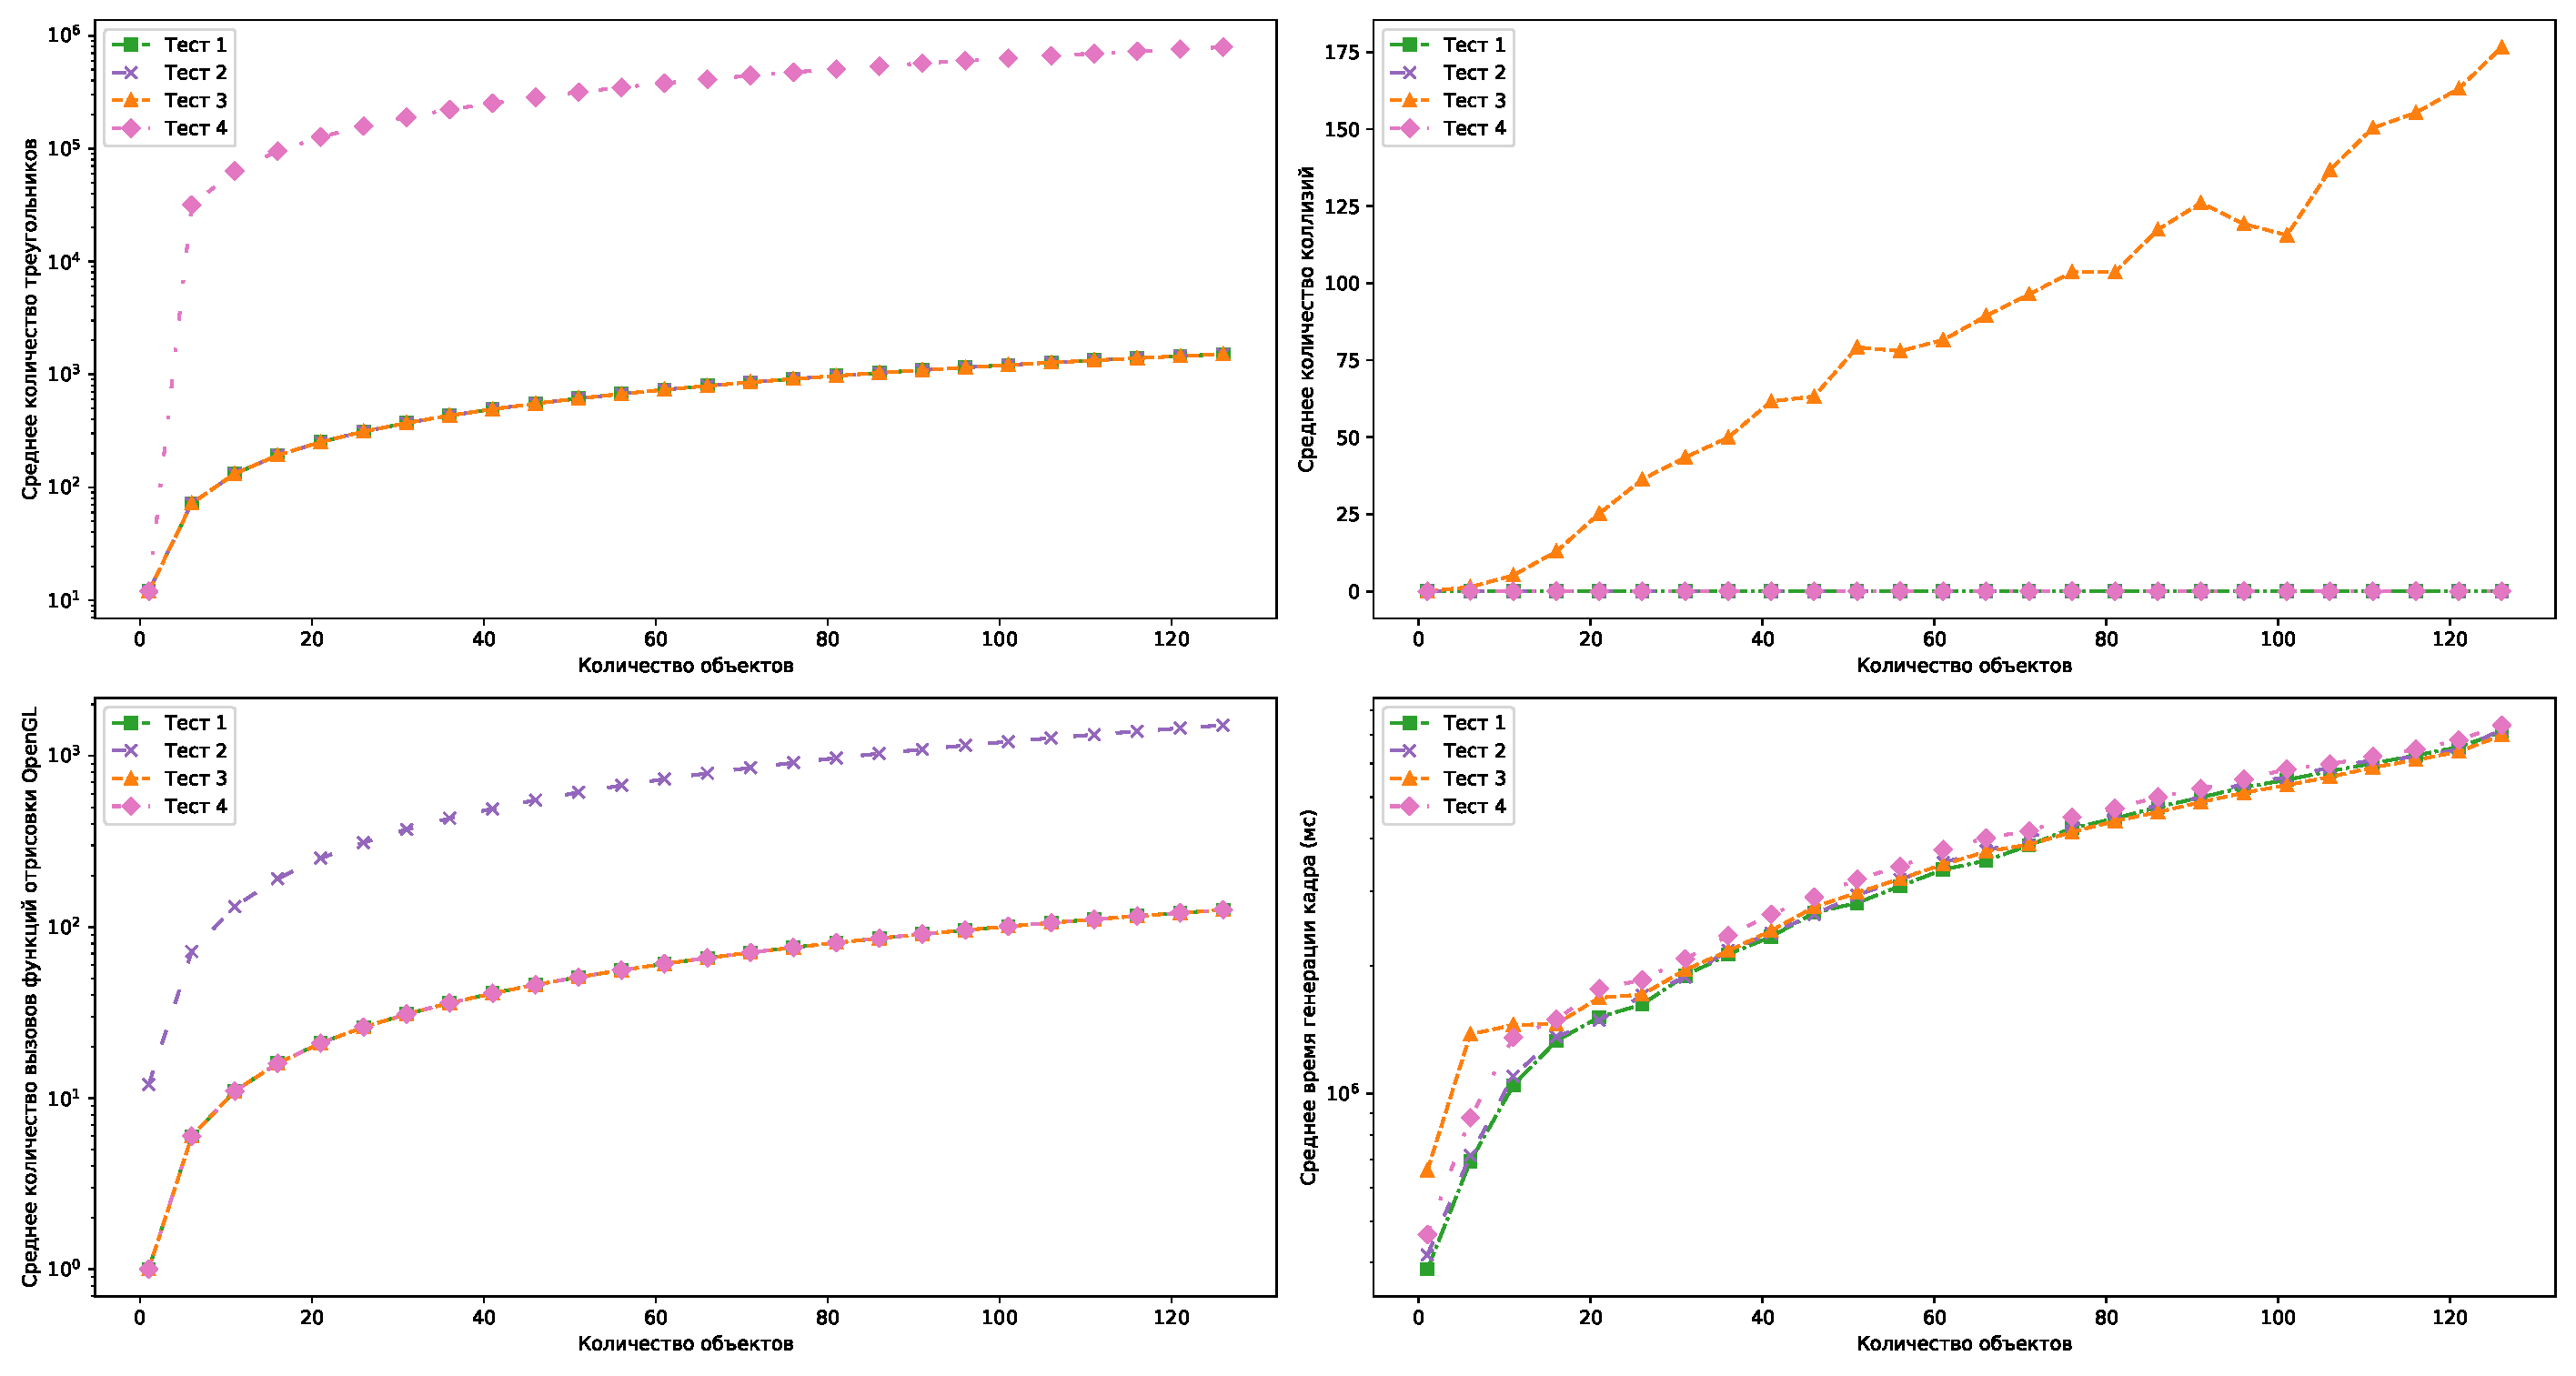
\includegraphics[width=\textwidth]{img/tests-1234.pdf}
	\caption{TODO}
	\label{fig:test1234}
\end{figure}

\begin{figure}[H]
	\centering
	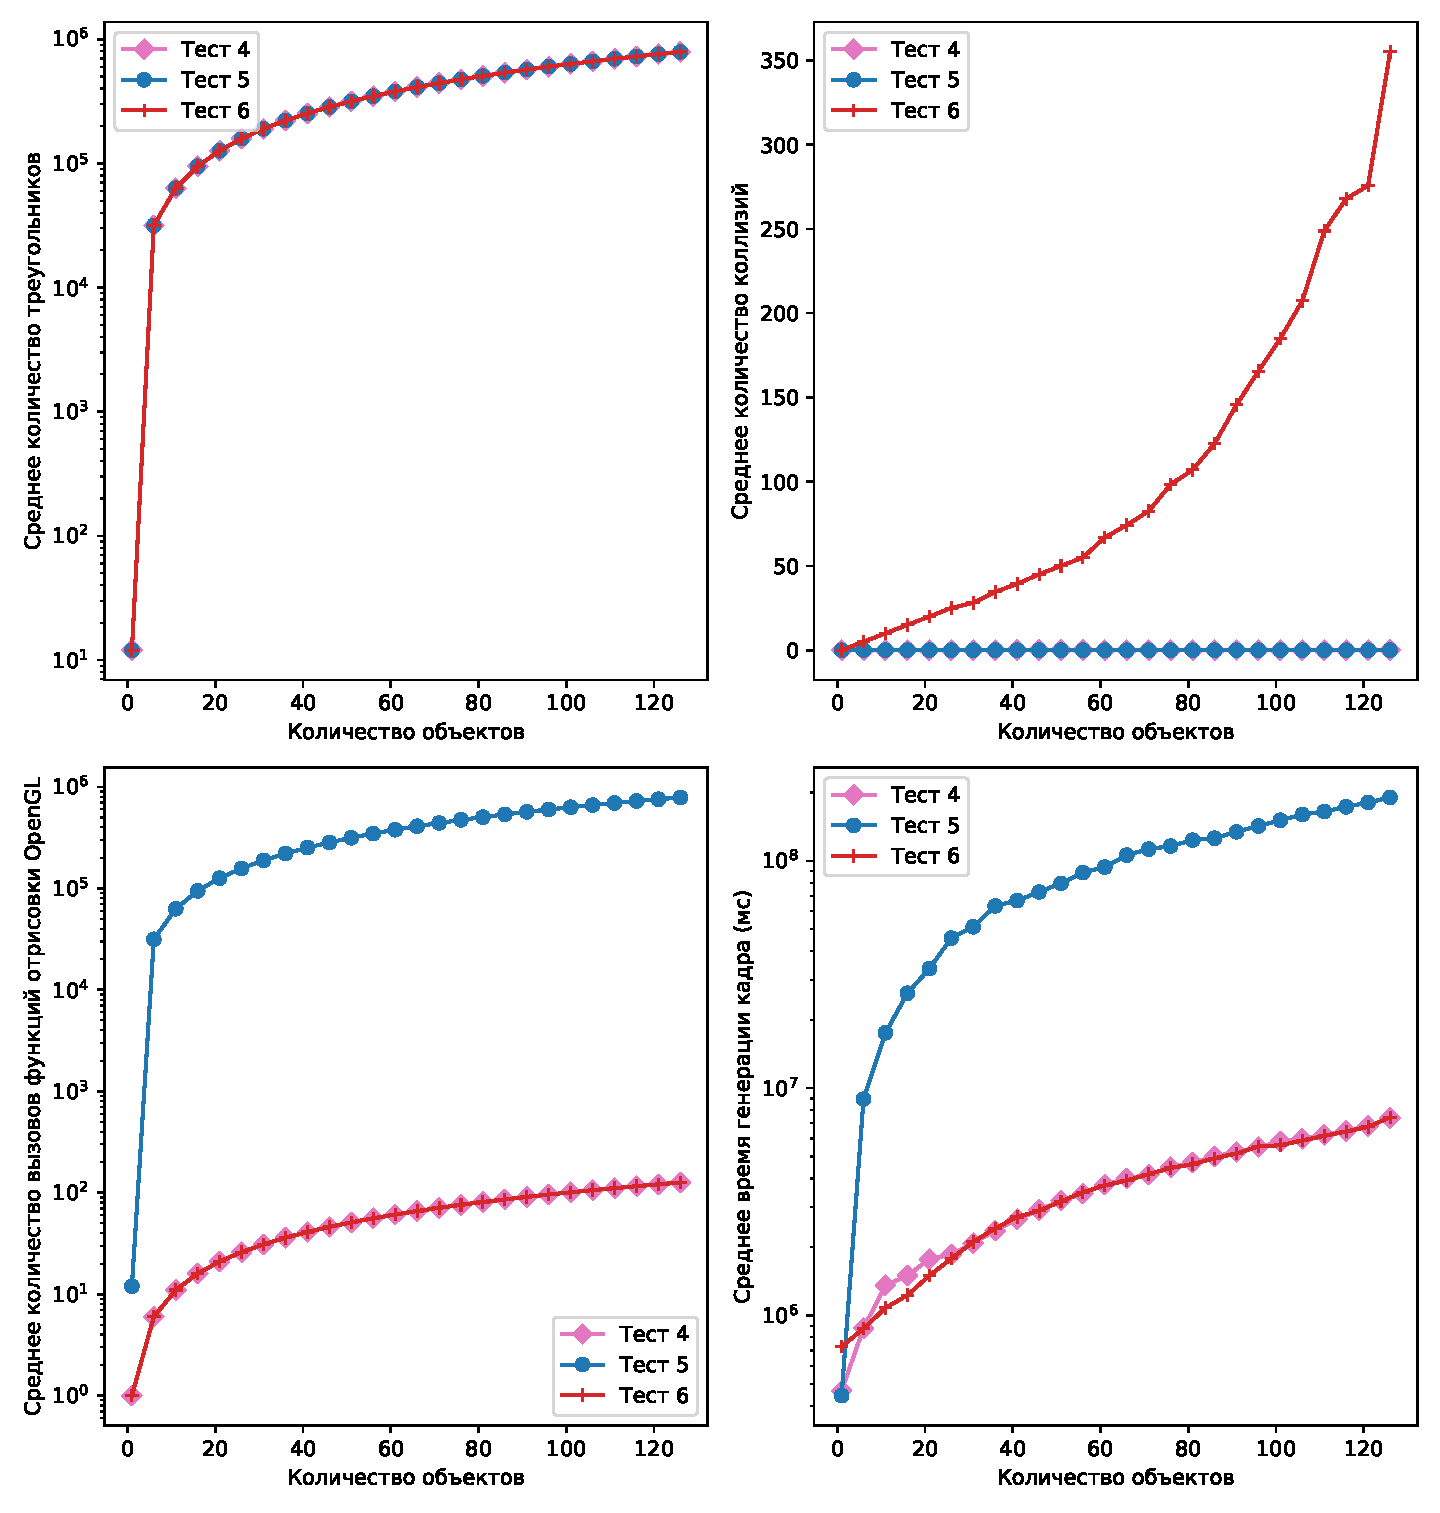
\includegraphics[width=\textwidth]{img/tests-456.pdf}
	\caption{TODO}
    \label{fig:test456}
\end{figure}

% \subsubsection{Вывод}

\subsection{Влияние типов объектов на скорость генерации кадра}

% \subsubsection{Вывод}

\subsection*{Вывод}

% Количественная оценка результатов
% Оказалось, что А во столько-то раз эффективнее Б на таких-то данных
